\documentclass{article}
\usepackage{listings}
\usepackage[utf8]{inputenc}
\usepackage{graphicx}
\renewcommand{\figurename}{Figura}
\usepackage{mathtools}
\usepackage{hyperref}


\title{Informe de Estadística en Física Experimental: Ejercicio 15 Guía 2}
\author{Andr\'es Babino}

\begin{document}
\maketitle
\section{Introducción}
El lenguaje utilizado para programar todas los ítems fue Python.
El código utilizado para generar los datos, gráficos y este mismo informe fue controlado con git, tiene licencia MIT y está almacenado en \url{https://github.com/ababino/efe}.

\section{Ítem a}
Abajo se encuentra el código de un programa que cuenta el número de éxitos de $n$ experimentos de Bernulli  con probabilidad de éxito $p$.
\begin{lstlisting}
def binomial_sample(n, p):
    """
    Takes a sample of size n from a binomial distribution with a success
    probability equal p. Returns the number of sucesses.
    """
    s = 0
    for i in xrange(n):
        x = random.random()
        if x < p:
            s += 1
    return s
\end{lstlisting}
El código está implementado en Python y usa el paquete estándar \textit{random}.

\section{Ítem b}
En la figura \ref{fig:itemb} se muestra un histograma que se obtiene utilizando la función anterior $1000$ veces.
El parámetro $p$ se tomó igual a $0.7$ y el parámetro $n$ igual a $15$.
Estos parámetros simulan un experimento hipotético en el que mil veces $15$ fotones impactan un detector con una eficiencia del $70\%$.
En negro se graficó la distribución de probabilidad de binomial $B(1000, 0.7)$.

\begin{figure}
\centering
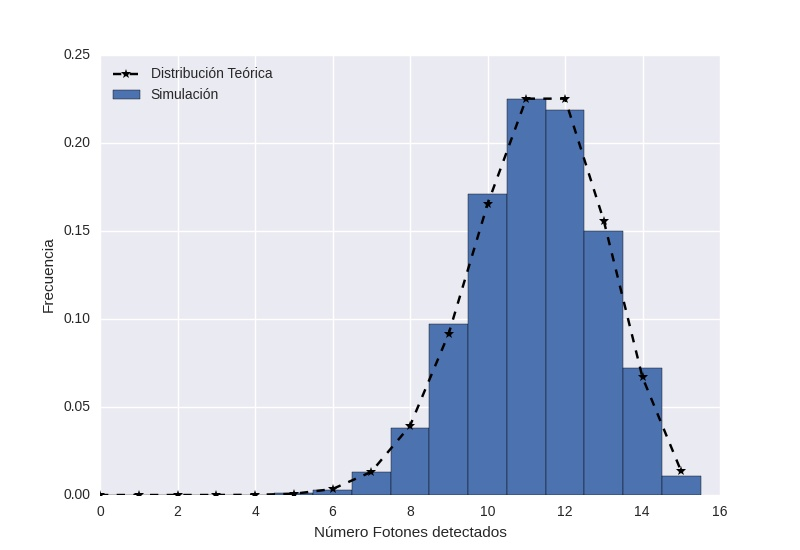
\includegraphics[width=0.75\textwidth]{figb.jpg}
\caption[]{Histograma del ítem b}
\label{fig:itemb}
\end{figure}

\section{Ítem c}
Ahora consideremos una fuente de intensidad media $I=15\ fot\ s^{-1}$.
La distribución de fotones emitidos en un intervalo de tiempo $t$ seguirá una distribución de Poisson.

$$\text{número\ de\ fotones} = \frac{(\lambda t)^k}{k!} e^{-\lambda t}$$

En la figura \ref{fig:poisson} vemos la distribución de Poisson cuando $\lambda=15$ y $t=0.001$.
Con estos parámetros la probabilidad de que no ocurra ningún evento es $del 98.51\%$ y la probabilidad de que ocurra un único evento es del $1.48\%$.
Estas dos probabilidades sumadas dan $99.99\%$  lo que quiere decir que la probabilidad de que sucedan dos o más eventos es $0.01\%$.
Vemos que la probabilidad de que ocurran 2 eventos es suficientemente pequeña como para suponer que no se observaran este tipo de eventos si repetimos el experimento $1000$ veces, es decir durante $1s$.
Es por esto que podemos simular la emisión de fotones como una sucesión de eventos binomiales.

\begin{figure}
\centering
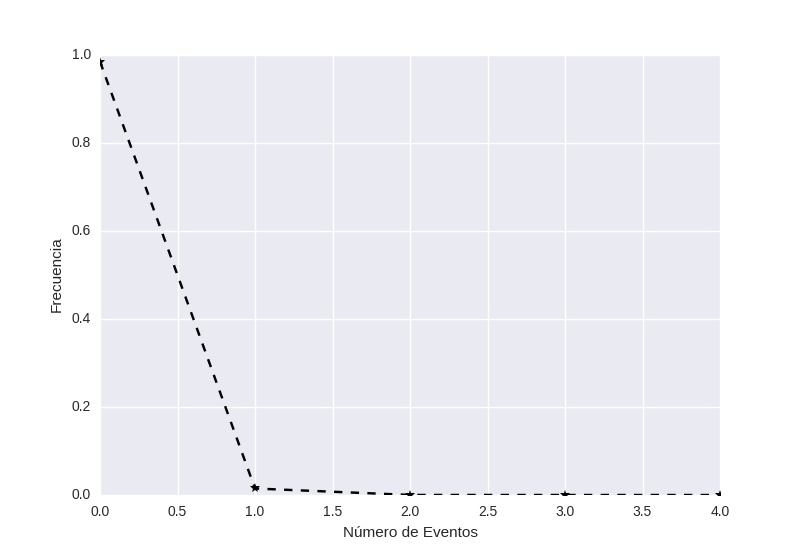
\includegraphics[width=0.75\textwidth]{poisson.jpg}
\caption[]{Distribución de probabilidad de Poisson con parámetro $\lambda=0.015$}
\label{fig:poisson}
\end{figure}

Con esto en mente utilizamos nuevamente el programa \textit{binomial\_sample} para simular una fuente con estas características.
En la figura \ref{fig:itemc} se observa el histograma de eventos simulados de esta manera y en linea negra la distribución de Poisson correspondiente. Se observa un buen acuerdo, lo que significa que la aproximación que hicimos es razonable.

\begin{figure}
\centering
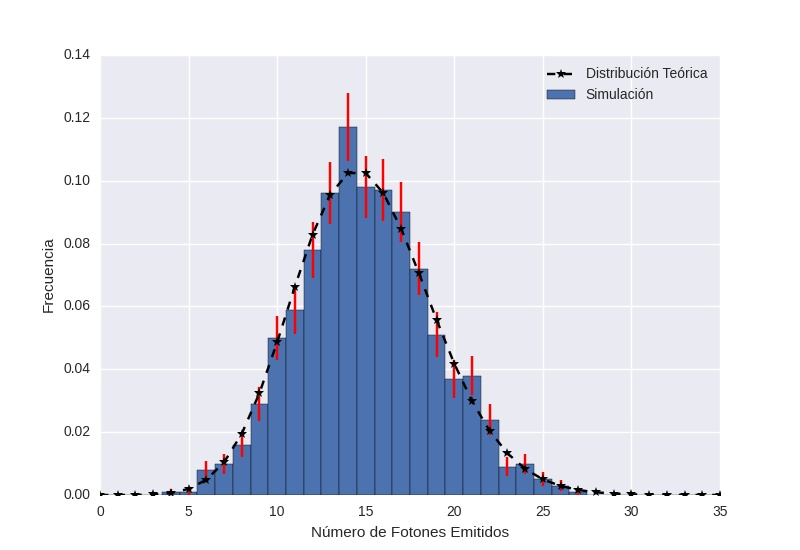
\includegraphics[width=0.75\textwidth]{figc.jpg}
\caption[]{Histograma del ítem c}
\label{fig:itemc}
\end{figure}

\section{Ítem d}
Ahora vamos a utilizar cada uno de los 1000 ensayos de emisión de fotones simulados en el ítem c como entrada para el detector simulado en el ítem b.
Lo que obtenemos es una simulación del número de fotones detectados por el detector que fueron emitidos por la fuente.
El histograma de esta simulación se puede ver en la figura  \ref{fig:itemd}.

La producción de fotones en la fuente sigue una distribución de Poisson y el número de fotones detectados dado el arribo de $n$ fotones sigue una distribución binomial.
Ahora nos preguntamos cuál será la distribución de fotones detectados dado el arribo de los fotones producidos con una distribución de Poisson.
La probabilidad de que se detecten $k$ fotones será:
$$
P(k) = \sum_{k=n}^{\infty} B_k(n, \epsilon) P_n(\lambda t)
$$
donde $B_k(n, \epsilon)$ es la distribución binomial que describe el proceso de medición y $P_n(\lambda t)$ es una distribución de Poisson que describe el proceso de producción de fotones.
Si escribimos la definición de estas distribuciones obtenemos:
$$
P(k) = \sum_{k=n}^{\infty} \frac{n!}{k!(n-k)!}\epsilon^k (1- \epsilon)^(n-k) \frac{(\lambda t)^n}{n!}e^{-\lambda t}
$$

Definiendo $m=n-k$ y sacando todo lo que no depende de $m$ fuera de la suma obtenemos:

$$
P(k) = \frac{\epsilon^k (\lambda t)^k e^{-\lambda t}}{k!} \sum_{m=0}^{\infty} \frac{[\lambda t(1- \epsilon)]^m}{m!}
$$

Escrito así el sumando es la definición de la exponencial $e^{\lambda t(1- \epsilon)}$.
Agrupando obtenemos:

$$
P(k) = \frac{(\epsilon \lambda t)^k}{k!} e^{-\epsilon \lambda t}
$$

Que es una distribución de Poisson con constante $\epsilon \lambda t$.
Por lo tanto para comparar nuestro histograma de la figura \ref{fig:itemd} debemos usar una distribución de Poisson con constante $10.5$.
En la figura \ref{fig:itemd} se ve en negro esta distribución y se observa que se corresponde con los datos simulados.


\begin{figure}
\centering
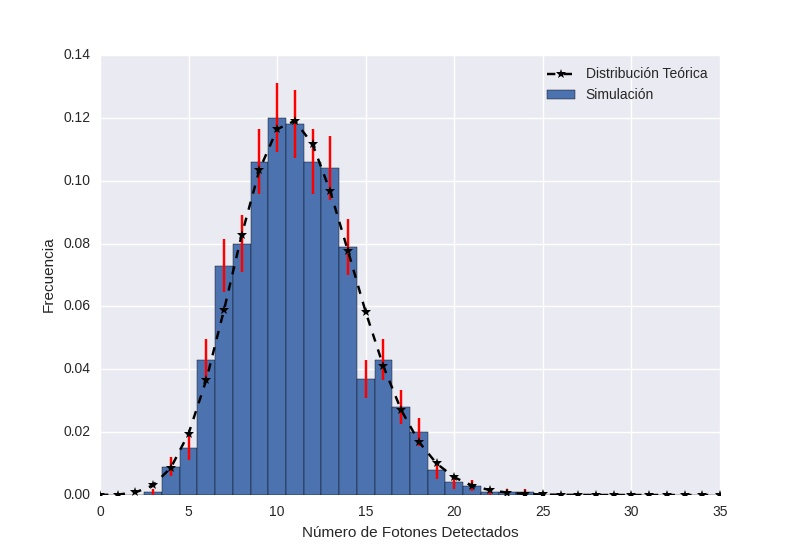
\includegraphics[width=0.75\textwidth]{figd.jpg}
\caption[]{Histograma del item d}
\label{fig:itemd}
\end{figure}

\section{Ítem e}

Con lo desarrollado en el ítem d podemos simular el mismo proceso utilizando el método del ítem c pero con una constante $10.5$.
Esto debería ser equivalente a la simulación del ítem anterior dado que hemos demostrado que la composición de un proceso de Poisson con uno Binomial es un proceso de Poisson.
Efectivamente en la figura \ref{fig:iteme} se observa esta simulación y se puede ver que también es consistente con la misma curva teórica indicando que los dos métodos para simular el proceso son equivalentes como hemos demostrado matemáticamente en el ítem anterior.

\begin{figure}
\centering
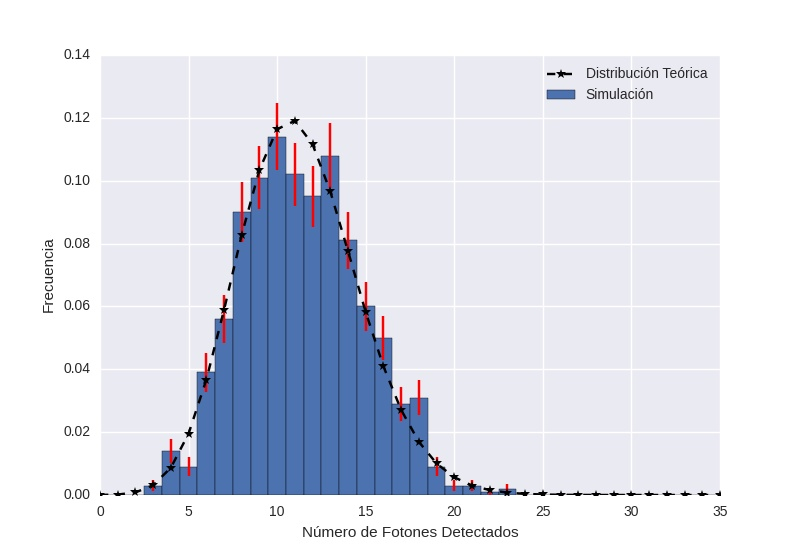
\includegraphics[width=0.75\textwidth]{fige.jpg}
\caption[]{Histograma del ítem e}
\label{fig:iteme}
\end{figure}

\section{Ítem f}
Todos los histogramas de este informe tiene barras de error.
En este ítem vamos a justificar el tamaño de las mismas.

Supongamos que para confeccionar un histograma utilizamos n datos (en todos los histogramas de este informe se usó $n=1000$).
Consideremos un casillero en particular de este histograma.
La probabilidad de que un determinado dato en ese casillero será un dado valor $p$.
Luego de realizar el histograma podemos estimar $p$ como el número de eventos, $k$, que efectivamente cayeron en esta realización en el casillero en cuestión sobre el numero de datos totales $n$.
Es decir que $\hat p = \frac{k}{n}$.
Considerando que la probabilidad $q$ de que un dato no caiga en el casillero en cuestión se puede estimar como $\hat q = 1 - \hat p$ vemos que estamos en presencia de un proceso binomial.
Entonces el número de datos que caen en un determinado casillero seguirá un distribución binomial de parámetros $n$ y $p$.
El desvío estándar de esta distribución se puede estimar como $\hat \sigma(k) = \sqrt{k (1 - \frac{k}{n})}$.

En el caso en el que $p\rightarrow 0$ se puede aproximar $\hat \sigma(k) = \sqrt{k}$.
Este caso es generalmente cuando el número de bines es suficientemente grande.
En esta situación la distribución binomial se puede aproximar por la distribución de Poisson.
Si este no es el caso estaremos sobre estimando el erro al hacer esta aproximación.


En todos los gráficos de este informe se usó un error poissoniano excepto en el histograma de la figura \ref{fig:itemb} que se uso el error binomial.





\end{document}
